\chapter{Background}
\label{chap:background}
In this chapter we describe the background techniques and tools used in our research. All tools were selected based on the ability to execute command-line using a script, the ability to export output reports, and the ability to fulfill the needs of our research.


\section{Mutation Testing}
\label{sec:background_mutation_testing}
Fault-based testing can be used as a coverage technique to demonstrate the absence of faults in a software system~\cite{DLS78, BSLS80}. Mutation testing makes use of fault-based testing by generating a set of mutants, each representing a possible fault in the software system. These mutants are then executed along with the test suite with hopes that the test suite can detect the mutant's fault. If the fault is detected this means that the test suite is effective enough to handle the detection of that specific bug. If the fault goes undetected then the test suite is lacking as it cannot detect that specific bug. Using the results of mutation testing it is possible to assess the adequacy of a test suite -- the effectiveness of the test suite of detecting bugs. Figure~\ref{fig:mutation_testing_overview} illustrates a generic process for mutation testing, the main components are mutation generation and mutation evaluation.

\begin{figure}[h!]
  \centering
  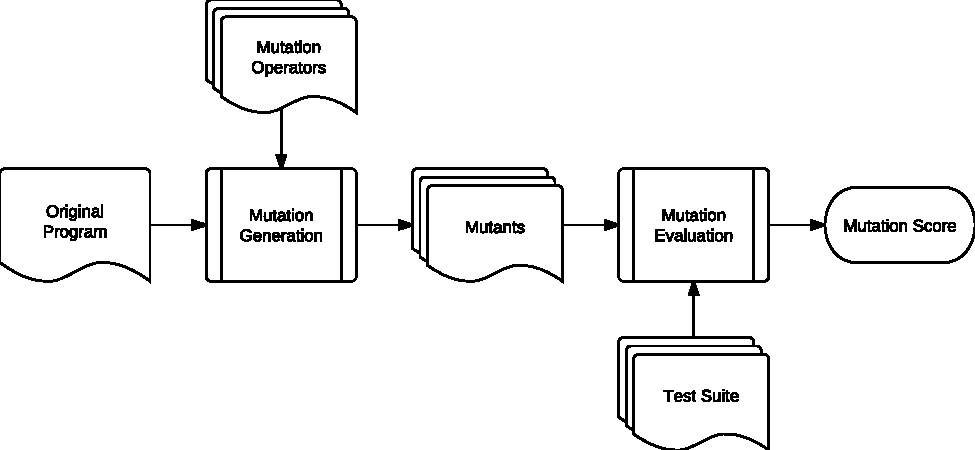
\includegraphics[width=14cm]{figures/mutation_testing_overview.pdf}
  \caption{A generic process for mutation testing.}
  \label{fig:mutation_testing_overview}
\end{figure}

Mutation testing uses a set of \emph{mutation operators} to generate faulty versions of a software system's source code called mutants. A mutation operator applies a transformation to a software artifact such that it now exhibits a fault (see Section~\ref{subsec:background_method_operators}~\&~\ref{subsec:background_class_operators} for examples). Mutation operators are designed based on existing fault taxonomy, such that the generate mutants that represent real faults. Studies have indicated that mutants could be used as substitutes for real faults with caution to external threats~\cite{ABLN06, NK11}.

The transformation is a small and single change as most bugs appear follow the \emph{\gls{cph}}~\cite{ABD+79} which suggests that developers write software that is nearly correct. The \emph{\gls{ceh}}~\cite{Off92} suggests that a large percent of complex faults can be detected if all the simple faults can be detected. These two hypothesis strengthen the use of simple small changes for mutation operators and why mutation testing is adequate for evaluating test suite effectiveness.

After all the mutants have been generated a testing approach is used to evaluate them against the test suite. If a mutant is detected by the test suite then the mutant is \emph{killed} otherwise it has \emph{survived}. There are some cases where the mutant generated is \emph{equivalent} such that the behaviour of the mutant is the same as the original system. These equivalent mutants pose a problem as they cannot be killed using the given test suite. Manual inspection of mutants to determine if they are equivalent is not feasible for a large number of mutants. A \emph{mutation score} is given to each source code unit based on the number of percentage of non-equivalent mutants they killed. The mutation score indicates how effective a test suite is at detecting faults in terms of mutation fault-based testing adequacy.

% TODO Maybe show a small example of equivalent mutants?

\begin{small}
\begin{center}
\emph{$\text{mutation score} = \frac{\text{killed mutants}}{\text{total mutants} - \text{equivalent mutants}}$}
\end{center}
\end{small}

Mutation testing has traditionally been used as a coverage technique to evaluate the effectiveness of test suites and provide confidence in the testing process~\cite{JH10}. For over 30 years, mutation testing has been applied to software written in programming languages including C~\cite{DM96, JH08}, Fortran~\cite{KO91} and Java~\cite{MKO02, BCD06}. Furthermore, mutation testing has also been applied to non-programming artifacts such as formal specification languages~\cite{ABM98}, markup languages~\cite{PO10} and spreadsheets~\cite{AE09}.

There are two major critique on mutation testing: equivalent mutants and performance. Schuler et al. proposes a solution in determining whether a surviving mutant is equivalent or not using impact analysis~\cite{SZ10}. Their approach observes the impact of the original program's execution against that of the mutant in respect to control flow and data. Their experiments showed that using statement coverage allowed them to achieved a classification precision of 75\% and a recall of 56\%. In their previous work they also considered the use of the impact of dynamic invariants to uncover equivalent mutants~\cite{SDZ09}. Offutt et al. used compiler optimization techniques and were able to detect about 10\% of equivalent mutations~\cite{OC94}. Mutation sampling can be used to reduce the evaluation efforts by only considering a random subset of the generated mutants~\cite{Bud80}. Untch et al. introduced a mutation runtime technique call \emph{Mutant Schema Generation} that represented all possible mutants in a single meta-program~\cite{UOH93}. Offutt et al. were able to perform mutation testing at the bytecode level, effectively avoiding recompilations of the generated mutants~\cite{OMK04}.


\subsection{Method-Level Operators}
\label{subsec:background_method_operators}
We look at the set of method-level mutation operators found in \emph{MuJava}~\cite{MOK05}, as they are well documented and designed. These mutation operators apply source transformations that modify expressions at the method-level. These operators can cause data to be slightly off, as well as adjusting the outcome of conditions. Figure~\ref{tab:method_operators} tabulates the method-level mutation operators~\cite{MO05a}.

\begin{table}[h]
  \centering
  \rowcolors{2}{gray!30}{gray!20}
  \begin{tabular}{|l|l|}
    \hline
    \rowcolor[RGB]{169,196,223}
    \textbf{Operator} & \textbf{Description} \\
    \hline AOR & Arithmetic Operator Replacement \\
    \hline AOI & Arithmetic Operator Insertion \\
    \hline AOD & Arithmetic Operator Deletion \\
    \hline ROR & Relational Operator Replacement \\
    \hline COR & Conditional Operator Replacement \\
    \hline COI & Conditional Operator Insertion \\
    \hline COD & Conditional Operator Deletion \\
    \hline SOR & Shift Operator Replacement \\
    \hline LOR & Logical Operator Replacement \\
    \hline LOI & Logical Operator Insertion \\
    \hline LOD & Logical Operator Deletion \\
    \hline ASR & Assignment Operator Replacement \\
    \hline
  \end{tabular}
  \caption{The set of method-level mutation operators for Java.}
  \label{tab:method_operators}
\end{table}

To illustrate the effects of a method-level operator, we can look at the \emph{Relational Operator Relational} (\texttt{ROR}) mutation operator. This transformation replaces a relational operator (i.e., \texttt{>}, \texttt{>=}, \texttt{==}, \texttt{!=}, \texttt{=<} or, \texttt{<}) with another type of relational operator (see Figure~\ref{fig:ROR_mutation}). See Figure~\ref{fig:AOI_mutation} for another example demonstrating the \emph{Arithmetic Operator Insertion} (\texttt{AOI}) mutation operator. The remaining set of method-level mutation operators function in a similar fashion except with other operators (i.e., conditional, shift, logical and, assignment).

\begin{figure}[h]
  \centering
  \begin{minipage}{6.5cm}
  \centering
  \footnotesize{\textbf{Correct Program}}
  \lstinputlisting[language=Java, literate={>}{{\textcolor{red}{>}}}{1}]{listings/mutation_example.java}
  \end{minipage}
  $\xrightarrow{\texttt{ROR}}$
  \begin{minipage}{6.5cm}
  \centering
  \footnotesize{\textbf{Mutant Program}}
  \lstinputlisting[language=Java, literate={>}{{\textcolor{red}{<}}}{1}]{listings/mutation_example.java}
  \end{minipage}
  \caption{Example application of the \texttt{ROR} method-level mutation operator.}
  \vspace{1mm}
  \footnotesize{In Figure~\ref{fig:ROR_mutation} the syntax being transformed using the \texttt{ROR} is red in the source listing.}
  \vspace{1mm}
  \label{fig:ROR_mutation}
\end{figure}

\begin{figure}[h]
  \centering
  \begin{minipage}{6.5cm}
  \centering
  \footnotesize{\textbf{Correct Program}}
  \lstinputlisting[language=Java, literate={this.limit}{{\textcolor{red}{\textbf{this}.limit}}}{10}]{listings/mutation_example.java}
  \end{minipage}
  $\xrightarrow{\texttt{AOI}}$
  \begin{minipage}{6.5cm}
  \centering
  \footnotesize{\textbf{Mutant Program}}
  \lstinputlisting[language=Java, literate={this.limit}{{\textcolor{red}{\textbf{this}.limit---}}}{12}]{listings/mutation_example.java}
  \end{minipage}
  \caption{Example application of the \texttt{AOI} method-level mutation operator.}
  \vspace{1mm}
  \footnotesize{In Figure~\ref{fig:AOI_mutation} the syntax being transformed using the \texttt{AOI} is red in the source listing.}
  \vspace{1mm}
  \label{fig:AOI_mutation}
\end{figure}


\subsection{Class-Level Operators}
\label{subsec:background_class_operators}
We look at the set of class-level mutation operators found in \emph{MuJava}~\cite{MOK05, MKO02}, as they are well documented and designed. These mutation operators apply source transformations that modify language features at the class-level. These operators can allow objects to behave in unexpected ways, as well as exposing design issues. Figure~\ref{tab:class_operators} tabulates the class-level mutation operators~\cite{MO05b}.

\begin{table}[h]
  \centering
  \rowcolors{2}{gray!30}{gray!20}
  \begin{tabular}{|c|l|l|}
    \hline
    \rowcolor[RGB]{169,196,223}
    \textbf{Group} & \textbf{Operator} & \textbf{Description} \\
    \hline \ding{172} & AMC & Access modifier change \\
    \hline \ding{173} & IHD & Hiding variable deletion \\
    \hline \ding{173} & IHI & Hiding variable insertion \\
    \hline \ding{173} & IOD & Overriding method deletion \\
    \hline \ding{173} & IOP & Overriding method calling position change \\
    \hline \ding{173} & IOR & Overriding method rename \\
    \hline \ding{173} & ISI & \texttt{super} keyword insertion \\
    \hline \ding{173} & ISD & \texttt{super} keyword deletion \\
    \hline \ding{173} & IPC & Explicit call to a parent's constructor deletion \\
    \hline \ding{174} & PNC & \texttt{new} method call with child class type \\
    \hline \ding{174} & PMD & Member variable declaration with parent class type \\
    \hline \ding{174} & PPD & Parameter variable declaration with child class type \\
    \hline \ding{174} & PCI & Type cast operator insertion \\
    \hline \ding{174} & PCC & Cast type change \\
    \hline \ding{174} & PCD & Type cast operator deletion \\
    \hline \ding{174} & PRV & Reference assignment with other comparable variable \\
    \hline \ding{174} & OMR & Overloading method contents replace \\
    \hline \ding{174} & OMD & Overloading method deletion \\
    \hline \ding{174} & OAC & Arguments of overloading method call change \\
    \hline \ding{175} & JTI & \texttt{this} keyword insertion \\
    \hline \ding{175} & JTD & \texttt{this} keyword deletion \\
    \hline \ding{175} & JSI & \texttt{static} modifier insertion \\
    \hline \ding{175} & JSD & \texttt{static} modifier deletion \\
    \hline \ding{175} & JID & Member variable initialization deletion \\
    \hline \ding{175} & JDC & Java-supported default constructor creation \\
    \hline \ding{175} & EOA & Reference assignment and content assignment replacement \\
    \hline \ding{175} & EOC & Reference comparison and content comparison replacement \\
    \hline \ding{175} & EAM & Acessor method change \\
    \hline \ding{175} & EMM & Modifier method change \\
    \hline
  \end{tabular}
  \caption{The set of class-level mutation operators for Java.}
  \vspace{1mm}
  \footnotesize{\emph{Table~\ref{tab:class_operators} shows the set of class-level mutation operators. The group column indicates the specific language feature of the mutation operator (\ding{172}: Encapsulation, \ding{173}: Inheritance, \ding{174}: Polymorphism, \ding{175}: Java-Specific Features).}}
  \vspace{1mm}
  \label{tab:class_operators}
\end{table}

To illustrate the effects of a class-level operator, we can look at the \emph{Member Variable Initialization Deletion} (\texttt{JID}) mutation operator. This transformation deletes an instance variables initialization (see Figure~\ref{fig:ROR_mutation}). See Figure~\ref{fig:AMC_mutation} for another example demonstrating the \emph{Access Modifier Change} (\texttt{AMC}) mutation operator. The remaining set of class-level mutation operators function by inserting, deleting and, changing certain elements in the class with respect to inheritance, polymorphism and, Java-specific features).

\begin{figure}[h]
  \centering
  \begin{minipage}{6.5cm}
  \centering
  \footnotesize{\textbf{Correct Program}}
  \lstinputlisting[language=Java, literate={Integer\ limit\ =\ new\ Integer(10)}{{{\textcolor{red}{Integer\ limit\ =\ \textbf{new}\ Integer(10)}}}}{31}]{listings/mutation_example.java}
  \end{minipage}
  $\xrightarrow{\texttt{JID}}$
  \begin{minipage}{6.5cm}
  \centering
  \footnotesize{\textbf{Mutant Program}}
  \lstinputlisting[language=Java, literate={Integer\ limit\ =\ new\ Integer(10)}{{{\textcolor{red}{Integer\ limit}}}}{13}]{listings/mutation_example.java}
  \end{minipage}
  \caption{Example application of the \texttt{JID} class-level mutation operator.}
  \vspace{1mm}
  \footnotesize{In Figure~\ref{fig:JID_mutation} the syntax being transformed using the \texttt{JID} is red in the source listing.}
  \vspace{1mm}
  \label{fig:JID_mutation}
\end{figure}

\begin{figure}[h]
  \centering
  \begin{minipage}{6.5cm}
  \centering
  \footnotesize{\textbf{Correct Program}}
  \lstinputlisting[language=Java, literate={public}{{\textbf{\textcolor{red}{public}}}}{6}]{listings/mutation_example.java}
  \end{minipage}
  $\xrightarrow{\texttt{AMC}}$
  \begin{minipage}{6.5cm}
  \centering
  \footnotesize{\textbf{Mutant Program}}
  \lstinputlisting[language=Java, literate={public}{{\textbf{\textcolor{red}{private}}}}{7}]{listings/mutation_example.java}
  \end{minipage}
  \caption{Example application of the \texttt{AMC} class-level mutation operator.}
  \vspace{1mm}
  \footnotesize{In Figure~\ref{fig:AMC_mutation} the syntax being transformed using the \texttt{AMC} is red in the source listing.}
  \vspace{1mm}
  \label{fig:AMC_mutation}
\end{figure}


\subsection{Mutation Testing Tools}
\label{subsec:background_mutation_tools}
In the last decade a number of mutation testing tools for the Java programming language have emerged~\cite{JH10}. Most of the tools have unique features that set them apart from one-another. Table~\ref{tab:mutation_tools} shows a number of Java mutation tools along with their features:

\begin{description}
  \item [Inception Year] the year the tool was released to the public
  \item [Generation-Level] mutation can be generated either at the source code or bytecode level. Source code mutation generation requires re-compilation, while bytecode does not.
  \item [Test Selection] test selection indicates which unit test cases are ran for each mutant. A naive based approach simply runs all the unit test cases, while convention based runs all tests based on a package/test name or defined annotations. Coverage based approach only runs unit test cases that are directly involved in the mutated source code, while a manual bases approach allows the user to specify each unit test case.
  \item [Mutant Insertion] generated mutants are stored and ran against the selected unit test cases. A naive approach stores the mutants on disk and creates a new \gls{jvm} for each mutant. A schmeta~\cite{UOH93} approach stores all the mutants in a single class, and the mutants are enabled through runtime flags one-at-a-time. An in-memory approach stores all the mutants in-memory which are then injected into the \gls{jvm} by creating a new classloader. An instrumentation approach stores the mutants in memory, but injects them into the \gls{jvm} directly using an instrumentation \gls{api}.
  \item [Method-Level] whether a tool has a set of \emph{traditional} method-level mutation operators as mentioned in Section~\ref{subsec:background_method_operators}.
  \item [Concurrency-Level] whether a tool has a set of concurrency-level mutation operators, those which mutate concurrency syntax to cause potential deadlocks, data races and more concurrency related bugs.
  \item [Class-Level] whether a tool has a set of object-oriented class-level mutation operators as mentioned in Section~\ref{subsec:background_class_operators}.
  \item [JUnit Support] whether a tool has support for JUnit test cases (de facto for unit testing Java~\cite{JUnit}.
  \item [Command-Line] whether a tool has support to be ran via a command-line interface.
  \item [Structured Output] whether a tool has support to output results in a structure format (i.e., \gls{xml}, etc \ldots)
  \item [Unit Scores] whether a tool indicates the mutation score of individual source code units (i.e., the mutation score of methods).
  \item [Open Source] whether a tool's source code is open source and freely available to modify.
  \item [Academic Tool] whether a tool was developed from an academic research group, otherwise industry or community developed.
  \item [Special Feature] whether a tools has a special feature that is unique in mutation testing.
\end{description}

\begin{landscape}
  \begin{table}[h]
    \centering
    \rowcolors{1}{gray!30}{gray!20}
    \begin{threeparttable}
      \begin{tabular}{|l|l|l|l|l|l|l|}
        \rowcolor[RGB]{169,196,223}
        \hline & \textbf{Jester~\cite{Jester}} & \textbf{MuJava~\cite{MOK05}} & \textbf{Jumble~\cite{Jumble}} & \textbf{Javalanche~\cite{SZ09}} & \textbf{Judy~\cite{MR10}} & \textbf{PIT~\cite{PIT}} \\
        \hline \cellcolor[RGB]{169,196,223} \textbf{Inception Year} & 2001 & 2004 & 2007 & 2009 & 2010 & 2011 \\
        \hline \cellcolor[RGB]{169,196,223} \textbf{Generation-Level} & Source Code & Bytecode & Bytecode & Bytecode & Source Code & Bytecode \\
        \hline \cellcolor[RGB]{169,196,223} \textbf{Test Selection} & Naive\tnote{f} & Manual & Convention & Coverage & Convention & Coverage \\
        \hline \cellcolor[RGB]{169,196,223} \textbf{Mutant Insertion} & Naive\tnote{f} & Schmeta & In-Memory & Schmeta & Schmeta\tnote{c} & Instrument \\
        \hline \cellcolor[RGB]{169,196,223} \textbf{Method-Level} & No & Yes & No & Yes & Yes & Yes \\
        \hline \cellcolor[RGB]{169,196,223} \textbf{Concurrency-Level} & No & No & No & Yes & No & No \\
        \hline \cellcolor[RGB]{169,196,223} \textbf{Class-Level} & No & Yes & No & No & Yes\tnote{b} & No \\
        \hline \cellcolor[RGB]{169,196,223} \textbf{JUnit Support} & Yes & No\tnote{c} & Yes & Yes & Yes & Yes \\
        \hline \cellcolor[RGB]{169,196,223} \textbf{Command-Line} & Yes & No & Yes & Yes & Yes & Yes \\
        \hline \cellcolor[RGB]{169,196,223} \textbf{Structured Output} & No & No & No & Yes & No & Yes \\
        \hline \cellcolor[RGB]{169,196,223} \textbf{Unit Scores} & No & No & No & Yes & No & No\tnote{g} \\
        \hline \cellcolor[RGB]{169,196,223} \textbf{Open Source} & Yes & No\tnote{d} & Yes & Yes & No & Yes \\
        \hline \cellcolor[RGB]{169,196,223} \textbf{Academic Tool} & No & Yes & No & Yes & Yes & No \\
        \hline \cellcolor[RGB]{169,196,223} \textbf{Special Feature} & No & No & No & Yes\tnote{e} & No & No \\
        \hline
      \end{tabular}
      \begin{tablenotes}
        \item[a] The Eclipse plugin has support for JUnit 3.
        \item[b] Limited set of class-level operators.
        \item[c] Iterative schmata (only allows a certain limit of mutants per iteration).
        \item[d] Limited basis to researchers.
        \item[e] Impact analysis to deal with equivalent mutants.
        \item[f] Best guess considering limited documentation.
        \item[g] The unit score could be calculated manually using structured output.
      \end{tablenotes}
    \end{threeparttable}
    \caption{Java mutation testing tools and their feature.}
    \vspace{1mm}
    \footnotesize{\emph{Table~\ref{tab:mutation_tools} shows a categorization of several Java mutation testing tools(table compiled using data from~\cite{PIT, MR10})}}
    \vspace{1mm}
    \label{tab:mutation_tools}
  \end{table}
\end{landscape}


\section{Machine Learning}
\label{sec:background_machine_learning}
Machine learning is a branch of artificial intelligence that primarily focuses on the ability to classify complex data. Given a set data with complex relationship within it, machine learning algorithms can attempt to uncover patterns that describe the data. With the uncovered patterns and relationships it then is possible to make intelligent predictions based on the data.

There are two types of machine learning algorithms for classification algorithms: \emph{supervised} and \emph{unsupervised} learning. The main difference between the two types of algorithms is whether one can properly classify some data prior to using the algorithm. In situations where nothing is known about the data set in terms of classification of the data then a unsupervised classification algorithm could be used. These types of algorithms generally aim to classify the data based on density or clusters (i.e., \emph{k}-mean clustering). The other type of algorithm, supervised learning, requires that an \emph{expert} can classify some of the data to use for \emph{training}. Using a supervised learning algorithm a model is created that describes the training data. Unclassified data can then be passed through the model to see what classification best fits the data.

If one does not have any idea of what the they are trying to classify, unsupervised learning is the best approach. It is not possible to categorize the data correctly, and incorrect categorization would only be detrimental to the classification. If it is possible to categorize the data then it becomes possible to perform supervised learning on the data. With correct categorization for the training data, future data can be classified on the constructed model from the training phase. In a sense unsupervised learning is more on exploratory need, while supervised learning is more on constructing a classifier.

In either case both learning algorithms require data to be classified. Dataset consist of a feature set of size \emph{n}. The power of machine learning comes of its ability to handle multiple dimensions of features for multiple dimensions of classification categories. For unsupervised learning datasets do not require a classification category. On the other hand the datasets for supervised learning require a pre-determined category.

Many areas of research have benefited from machine learning such as the data mining~\cite{WFH11}, computer vision~\cite{Her03}, biology~\cite{OLP08}, business~\cite{Her00}, health sciences~\cite{Kon01} amongst many others areas. Furthermore, most companies that offer a complex recommendation system utilize machine learning techniques. For example in 2006, \emph{Netflix} challenged the computer science, data mining and machine learning communities to develop a system that exceed its own recommendation system~\cite{BL07}.


\subsection{Support Vector Machine}
\label{subsec:background_support_vector_machine}
A \gls{svm} is an example of a linear discrimination machine learning technique and assumes that ``...\emph{instances of a class are linearly separable from instances of other classes}''~\cite{ALP04}. Traditionally, \gls{svm}s have been used for two-group classification problems~\cite{CV95} but have also been generalized to \emph{n}-group classification problems. The dataset used in \gls{svm} is applied to a \emph{feature space} that consists of a set of \emph{vectors} (a row of data in the dataset), with each vector containing a set of \emph{attributes} (the values that define the vector). In Figure~\ref{fig:SVM_margin} we have a \gls{svm} example with each vector having two predictor variables (\emph{x} and \emph{y} coordinates). A \gls{svm} attempts to find the maximum margin space between support vectors of opposite categories, which results in the optimal hyperplane. The optimal hyperplane is chosen over other as ``Intuitively, we would expect this boundary to generalise well as opposed to the other possible boundaries.''~\cite{Gun98}.

\begin{figure}[h]
  \centering
  \fbox{\subfloat[][\gls{svm} separated with a small margin between support vectors]{
    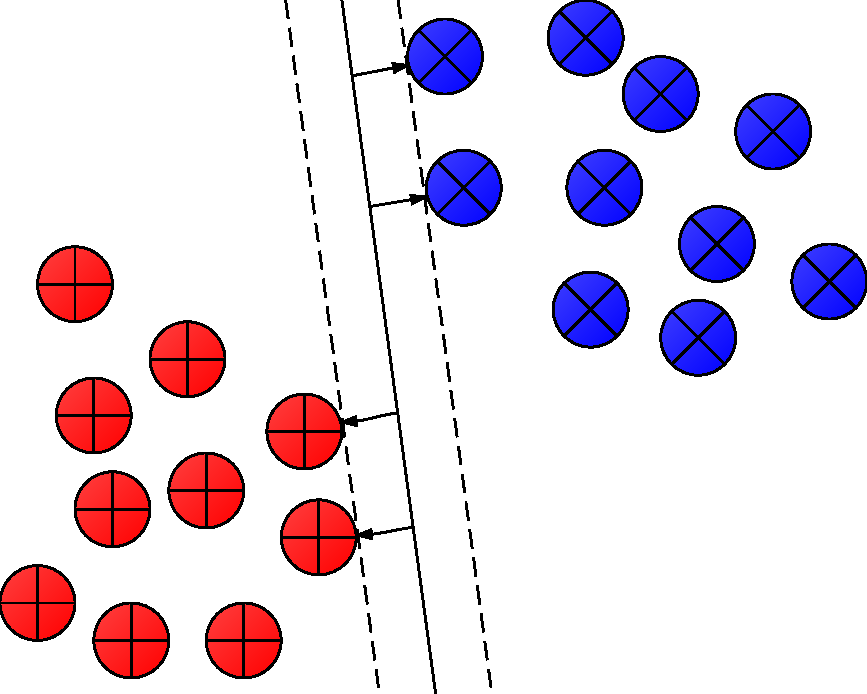
\includegraphics[width=5.5cm]{figures/SVM_small_margin.pdf}
    \label{fig:SVM_small_margin}
  }}
  \qquad
  \fbox{\subfloat[][\gls{svm} separated with a maximum margin between support vectors]{
    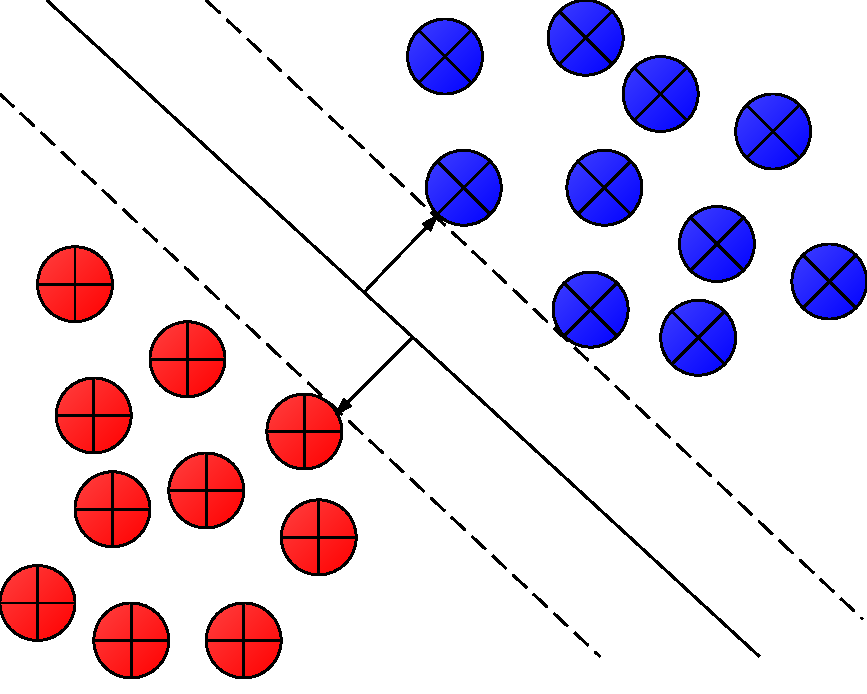
\includegraphics[width=5.5cm]{figures/SVM_maximum_margin.pdf}
    \label{fig:SVM_maximum_margin}
  }}
  \caption{Difference between small and maximum margins between support vectors.}
  \vspace{1mm}
  \footnotesize{As we can see in Figure~\ref{fig:SVM_margin} two simple example of \gls{svm}s are illustrated. There are two categories in the feature space with a solid line separating them, this is called the \emph{hyperplane}. The dotted lines represent the distance to the closest vector from the hyperplane, the distance between both dotted lines is also called the \emph{margin}. \emph{Support vectors} are the vectors that are touching the margin. The goal of a \gls{svm} is to maximizing the distance between support vectors of opposite categories using the hyperplane. There is a clear difference in the distance separating support vectors in the above examples, with the maximum margin~\subref{fig:SVM_maximum_margin} being a better solution then the small margin~\subref{fig:SVM_small_margin}.}
  \vspace{1mm}
  \label{fig:SVM_margin}
\end{figure}

In some cases a linear separation is not possible in the feature space, for example in Figure~\ref{fig:SVM_non-linear_kernel}. It is possible to map the vectors to a higher dimension such that the feature space now becomes linearly separable. The separating hyperplane is always of \emph{n}-1 dimensions (for example, two dimensional data is separated with a 1 dimensional line). Over-fitting can lower the ability of a classifier to generalize. \gls{svm} handle this first with the maximum margin distance which allows some flexibility in adding new vectors to the feature space. Secondly, the concept of \emph{cost} is also present in \gls{svm}. If there is a low cost then the the \gls{svm} will allow some mis-classifications (within a distance from the hyperplane using a function of cost). A higher cost value will reduce the number of mis-classifications, but may create a model that does not generalize outside of the training data.

\begin{figure}[h]
  \centering
  \fbox{\subfloat[][\gls{svm} separated with a small margin between support vectors]{
    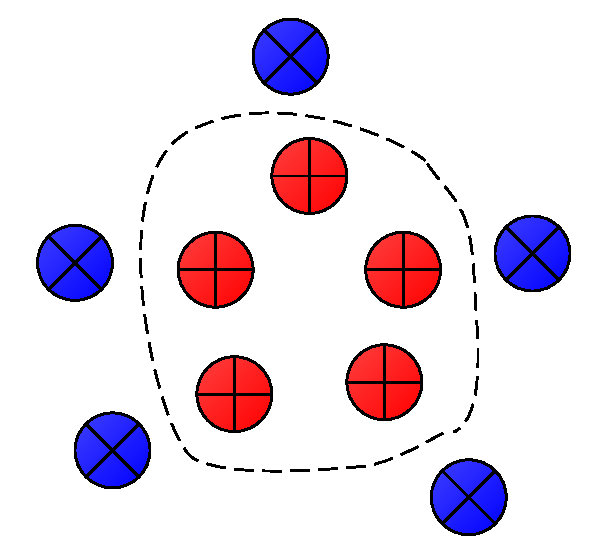
\includegraphics[width=5.5cm]{figures/SVM_non-linear.pdf}
    \label{fig:SVM_non-linear}
  }}
  $\xrightarrow{\texttt{Kernel Function}}$
  \fbox{\subfloat[][\gls{svm} separated with a maximum margin between support vectors]{
    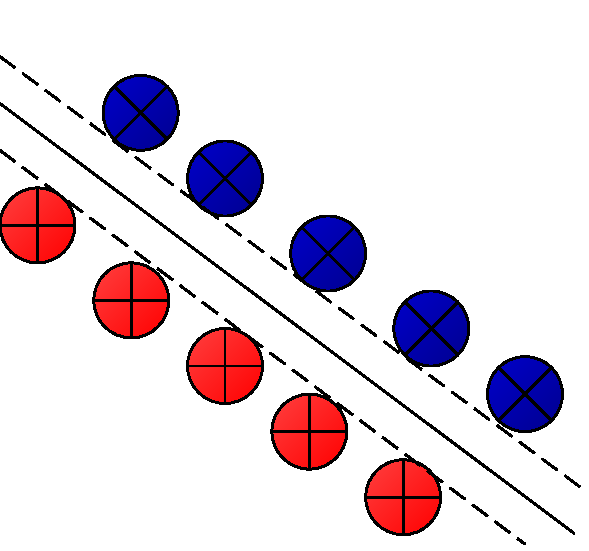
\includegraphics[width=5.5cm]{figures/SVM_kernel_function.pdf}
    \label{fig:SVM_kernel_function}
  }}
  \caption{Linearly separating non-linear data using a kernel function.}
  \vspace{1mm}
  \footnotesize{As we can see in Figure~\ref{fig:SVM_non-linear_kernel} two example of \gls{svm}s are illustrated. A non-linear hyperplane is required in~\subref{fig:SVM_non-linear} to properly separate the two categories. \gls{svm}s attempt to linearly separate the feature space, in this case it is possible to \emph{map} the vectors to a higher dimension using a \emph{kernel function}. In the above example a kernel function is used to map~\subref{fig:SVM_non-linear} to~\subref{fig:SVM_kernel_function} which results in a higher dimension such that each vector now has a \emph{radius} value (distance from the center). As we can see in~\subref{fig:SVM_kernel_function} it is now linearly separable when the feature space is mapped to a higher dimension (from two-dimensions to three-dimensions).}
  \vspace{1mm}
  \label{fig:SVM_non-linear_kernel}
\end{figure}


\section{Metrics}
\label{sec:background_metrics}
Metrics are measurements of a system, in which they can provide insight in describing the system. Goodman defines software metrics as ``\emph{The continuous application of measurement-based techniques to the software development process and its products to supply meaningful and timely management information, together with the use of those techniques to improve that process and its products}''~\cite{Goo93}. Having the ability to measure a system and use those measurement for future considerations is a large benefit of metrics. For software systems there are plentiful metrics that can be acquire and used. In most cases anything that can be measured can very well be used as a metrics.


\subsection{Source Code Metrics}
\label{subsec:background_source_code_metrics}
Software metrics can be used to measure a number of qualities of a software system. In particular, source code metrics give insight into structural aspects of the system including it's complexity, size, as well as object-oriented attributes~\cite{McCa76, Kan02, HWY09, Hend95, SRD12}. Chidamber et al. presented a suite of object-oriented metrics~\cite{CK94}, around the same time Abreu et al. also presented the MOOD object-oriented suite~\cite{AC94}. Source code metrics are typically extracted from the source code using static analysis techniques. Some metrics like \emph{defect density} make use of external bug reports along with the source code to indicate problematic modules~\cite{FP98}. In other cases software metrics might only be observable during the execution of the system in cases where dynamic/runtime metrics are considered~\cite{SS08}. Table~\ref{tab:source_metrics} presents a number of source code metrics that measure the structure of a software system.

\begin{table}[h]
  \centering
  \rowcolors{2}{gray!30}{gray!20}
  \begin{tabular}{|l|l|l|}
    \hline
    \rowcolor[RGB]{169,196,223}
    \textbf{Metric} & \textbf{Description} & \textbf{Scope} \\
    \hline MLOC & Method lines of code & Method \\
    \hline NBD & Nested block depth & Method \\
    \hline VG & McCabe cyclomatic complexity & Method \\
    \hline PAR & Number of parameters & Method \\
    \hline NORM & Number of overridden methods & Class \\
    \hline NOF & Number of attributes & Class \\
    \hline NSC & Number of children & Class \\
    \hline DIT & Depth of inheritance tree & Class \\
    \hline LCOM & Lack of cohesion of methods & Class \\
    \hline NSM & Number of static methods & Class \\
    \hline NOM & Number of methods & Class \\
    \hline SIX & Specialization index & Class \\
    \hline WMC & Weighted method per class & Class \\
    \hline NSF & Number of static attributes & Class \\
    \hline SMLOC & Sum MLOC of methods & Class \\
    \hline SNBD & Sum NBD of methods & Class \\
    \hline SVG & Sum VG of methods & Class \\
    \hline SPAR & Sum PAR of methods & Class \\
    \hline AMLOC & Average MLOC of methods & Class \\
    \hline ANBD & Average NBD of methods & Class \\
    \hline AVG & Average VG of methods & Class \\
    \hline APAR & Average PAR of methods & Class \\
    \hline
  \end{tabular}
  \caption{The set of source code metrics used in our research.}
  \vspace{1mm}
  \footnotesize{\emph{Table~\ref{tab:source_metrics} shows the set of metrics used in our research with respect to what source code unit scope they are connected with. Class-level source metrics measure object-oriented interactions and structural aspects for classes. Method-level source metrics measure method complexity and size.}}
  \vspace{1mm}
  \label{tab:source_metrics}
\end{table}


\subsection{Test Suite Metrics}
\label{subsec:background_test_suite_metrics}
Test suite metrics can be gathered using similar technique to those used in the gathering of source code metrics. There is less research and metrics in this area. In our research, we consider JUnit test cases as an aspect related to test suite metrics. Test case units still behave as source code, thus the complexity and size of test cases can be used as an observable metric. As mentioned in Section~\ref{sec:introduction_motivation}, coverage metrics can also assess what parts of the source code are exercise by the test suite~\cite{ZHM97}. Table~\ref{tab:test_suite_source_metrics} presents a set of test suite metrics that measure the complexity and size of the test suite for the \gls{sut}. Table~\ref{tab:test_suite_coverage_metrics} presents a set of test suite metrics that measure the coverage of the test suite for the \gls{sut}.

\begin{table}[h]
  \centering
  \rowcolors{2}{gray!30}{gray!20}
  \begin{tabular}{|l|l|}
    \hline
    \rowcolor[RGB]{169,196,223}
    \textbf{Metric} & \textbf{Description} \\
    \hline STMLOC & Sum MLOC of test methods \\
    \hline STNBD & Sum NBD of test methods \\
    \hline STVG & Sum VG of test methods \\
    \hline STPAR & Sum PAR of test methods \\
    \hline ATMLOC & Average MLOC of test methods \\
    \hline ATNBD & Average NBD of test methods \\
    \hline ATVG & Average VG of test methods \\
    \hline ATPAR & Average PAR of test methods \\
    \hline
  \end{tabular}
  \caption{The set of test suite source code metrics used in our research.}
  \vspace{1mm}
  \footnotesize{\emph{Table~\ref{tab:test_suite_source_metrics} shows the set of metrics used in our research with respect to what source code unit scope they are connected with. Class-level source metrics measure object-oriented interactions and structural aspects for classes. Method-level source metrics measure method complexity and size.}}
  \vspace{1mm}
  \label{tab:test_suite_source_metrics}
\end{table}

\begin{table}[h]
  \centering
  \rowcolors{2}{gray!30}{gray!20}
  \begin{tabular}{|l|l|}
    \hline
    \rowcolor[RGB]{169,196,223}
    \textbf{Metric} & \textbf{Description} \\
    \hline BCOV & Basic blocks covered in code unit \\
    \hline BTOT & Total basic blocks for code unit \\
    \hline NOT & Number of tests \\
    \hline
  \end{tabular}
  \caption{The set of test suite coverage metrics used in our research.}
  \vspace{1mm}
  \footnotesize{\emph{Table~\ref{tab:test_suite_coverage_metrics} shows a set of test suite metrics used in our research with respect to the coverage provided on the \gls{sut}. \emph{Basic block} is an atomic set of instructions, which can be used as a coverage measure.}}
  \vspace{1mm}
  \label{tab:test_suite_coverage_metrics}
\end{table}
